\chapter{Sistema de adquisición de datos DAQ}

  \section{Visión general de la comunicación serial}

    Con frecuencia, un sistema necesita comunicarse con otro que no reside en el mismo dispositivo. Para reducir el número de pines de I/O y el cableado externo, los dos sistemas pueden transferir datos a través de una única línea serial, bit a bit. El sistema transmisor realiza la conversión de paralelo a serie y, a continuación, envía los datos serie a través de una única línea. El sistema receptor realiza la conversión serie a paralelo y restaura los datos paralelos originales.

    La comunicación serial puede utilizarse tanto para transferir datos a alta velocidad como a baja velocidad. En una interfaz de alta velocidad, como USB y gigabit Ethernet, la velocidad de transmisión de datos puede alcanzar varios cientos de millones de bits por segundo o más. 

    En una interfaz de baja velocidad, la velocidad de transmisión de datos oscila entre varios miles y varios cientos de miles de bits por segundo. Es adecuada para la mayoría de los periféricos de I/O generales y para tareas de adquisición y control de datos. Dado que la velocidad de datos es mucho más lenta que la velocidad de reloj de una FPGA, estos esquemas pueden ser realizados por los elementos lógicos genéricos de una FPGA. A continuación se discuten los esquemas UART y SPI.

	\section{Controlador UART}

    La comunicación serial utiliza una única línea de datos para intercambiar información entre dos sistemas. El sistema transmisor convierte los datos paralelos en un flujo serie y el sistema receptor vuelve a ensamblar los datos serie en su formato paralelo original. El esquema más utilizado es el UART, (Universal Asynchronous Receiver and Transmitter) o receptor y transmisor asíncrono universal en español.

    \subsection{Visión general}

    Un controlador UART básico incluye un transmisor y un receptor. El transmisor es un registro de corrimiento especial que carga datos en paralelo y luego los desplaza bit a bit a una velocidad específica. El receptor, por su parte, desplaza los datos bit a bit y los vuelve a ensamblar. La línea serial es 1 cuando está inactiva. La transmisión comienza con un bit de inicio, que es 0, seguido de bits de datos y un bit de paridad opcional, y termina con bits de parada, que son 1. El número de bits de datos puede ser 6, 7 u 8. El bit de paridad opcional se utiliza para la detección de errores. Para paridad impar, se pone a 0 cuando los bits de datos tienen un número impar de 1's. Para paridad par, se pone a 0 cuando los bits de datos tienen un número par de 1's. El número de bits de parada puede ser 1, 1,5 ó 2. En la Figura \ref{fig:uart_transmission} se muestra la transmisión con ocho bits de datos, sin paridad y un bit de parada. Observe que el LSB de la palabra de datos se transmite primero.

    \begin{figure}[hbtp]
      \centering
      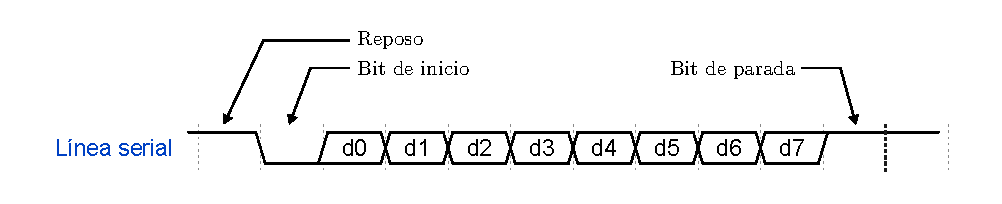
\includegraphics[width=0.95\textwidth]{uart_transmission}
      \caption{Diagrama de la transmisión de un byte serial con UART.}
      \label{fig:uart_transmission}
    \end{figure}

    A través de la línea serial no se transmite información de reloj. Antes de iniciar la transmisión, el transmisor y el receptor deben acordar de antemano una serie de parámetros, que incluyen la velocidad en baudios (es decir, el número de bits por segundo), el número de bits de datos y bits de parada, y el uso del bit de paridad. Con los parámetros predeterminados, el receptor utiliza un esquema de sobremuestreo para recuperar los bits de datos. Las velocidades en baudios más utilizadas son 9,600 y 19,200 baudios.

    \subsection{Procedimiento de sobremuestreo}

    La velocidad de muestreo más utilizada es 16 veces la velocidad en baudios, lo que significa que cada bit serie se muestrea 16 veces. Para un enlace de comunicación con N bits de datos y M bits de parada, el esquema de sobremuestreo funciona de la siguiente manera:
    
    \begin{enumerate}
      \item Espera hasta que la señal entrante se convierta en 0, el comienzo del bit de inicio, y luego comienza a contar los pulsos de muestreo.
      \item Cuando el contador llegue a 7, la señal entrante alcanzará el punto medio del bit de inicio. Limpia el contador a 0 y reinícialo.
      \item Cuando el contador llegue a 15, la señal entrante habrá avanzado un bit y alcanzará el punto medio del primer bit de datos. Obtén su valor, desplázalo a un registro y reinicia el contador.
      \item Repite el paso 3 N–1 veces más para obtener los bits de datos restantes.
      \item Si se utiliza el bit de paridad opcional, repite el paso 3 una vez para obtener el bit de paridad.
      \item Repite el paso 3 M veces más para obtener los bits de parada.
    \end{enumerate}

    El esquema de sobremuestreo realiza básicamente la función de una señal de reloj. En lugar de utilizar el flanco ascendente para indicar cuándo es válida la señal de entrada, utiliza los pulsos de muestreo para estimar el punto medio de cada bit. Aunque el receptor no tiene información sobre el momento exacto de inicio del bit, la estimación puede estar desviada como máximo en $1/16$. Las siguientes recuperaciones de bits de datos también se desvían como máximo de $1/16$ del punto medio. Debido al sobremuestreo, la velocidad en baudios sólo puede ser una pequeña fracción de la velocidad de reloj del sistema, por lo que este esquema no es apropiado para una velocidad de datos alta.


    \subsection{Diseño conceptual}

      El diagrama de alto nivel de un sistema UART se muestra en la Figura \ref{fig:uart_diagram}. Consiste en tres componentes principales. El generador de la tasa de baudios genera una señal de sobremuestreo. El receptor realiza la conversión de serie a paralelo y el transmisor realiza la conversión de paralelo a serie.

    \begin{figure}[h!]
      \centering
      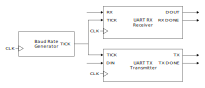
\includegraphics[width=0.8\textwidth]{uart_diagram}
      \caption{Diagrama de bloques de una controlador UART completo.}
      \label{fig:uart_diagram}
    \end{figure}

    \subsection{Generador de la tasa de baudios}

    El generador de la tasa de baudios genera una señal de muestreo cuya frecuencia es exactamente 16 veces la tasa de baudios designada para el UART. Para evitar la creación de un nuevo dominio de reloj y violar el principio de diseño síncrono, la señal de muestreo debe funcionar como pulsos de habilitación en lugar de la señal de reloj para el receptor UART.

    El generador de la tasa de baudios es un contador programable y el código HDL se muestra en el Código \ref{cod:baud_gen}. El código es un contador mod$-m$ parametrizado que se reinicia cada vez que el contador llega a un valor determinado. Por ejemplo para una tasa de 19,200 baudios, la tasa de muestreo tiene que ser de 307,200 (es decir, 19,200 $\times$ 16) pulsos por segundo. Dada una frecuencia del reloj de sistema de 50 MHz, el generador de la tasa de baudios necesita un contador mod-163, $\left( \frac{50 \times 10^{6}}{19200 \times 16} \right)$, en el cual se genera un pulso de ciclo de reloj cada 163 ciclos de reloj del sistema.

    \subsection{Receptor UART}

    \subsection{Transmisor UART}

	\section{Controlador SPI}

    El estándar SPI (Serial Peripheral Interface) o Interfaz Periférica Serial en español, es un protocolo de transferencia de datos en serie desarrollado originalmente por Motorola a principios de los 80. El bus SPI se compone de tres líneas, dos de ellas para transmitir y recibir datos en serie, y una para la señal de reloj. Se pueden conectar al bus un dispositivo maestro y varios dispositivos esclavos. El maestro genera la señal de reloj e inicia la transferencia de datos. El estándar SPI se utiliza ampliamente en sistemas embebidos para conectar módulos periféricos. \cite{Chu2018}, \cite{Chu2008}

    \subsection{Visión general}

    El estándar SPI especifica el protocolo que intercambia datos entre dos dispositivos a través de líneas seriales. En lugar de utilizar el esquema de sobremuestreo de UART, la interfaz SPI incluye una tercera línea para controlar el desplazamiento y el muestreo de los datos seriales. Las actividades se realizan en el flanco de transición de esta señal. Su función es similar a la señal de reloj de un sistema síncrono, por lo que esta línea se denomina reloj SPI.

    A diferencia de la configuración UART, en la que dos sistemas son simétricos y ambos pueden iniciar una transmisión, el estándar SPI utiliza una configuración maestro-esclavo. El maestro controla el funcionamiento general y genera la señal de reloj SPI. Sólo el maestro puede iniciar una transferencia de datos.

    A pesar de su nombre, el reloj SPI no es un reloj de sistema real y no debe utilizarse para controlar ningún registro directamente. La velocidad del reloj del sistema del controlador SPI es mucho más rápida que la velocidad del reloj SPI. Desde el punto de vista del controlador SPI, el reloj SPI es sólo otra señal de control.

    \subsection{Arquitectura del controlador}

    El diagrama conceptual de un bus SPI con dos dispositivos se muestra en la Figura \ref{fig:spi_diagram}. Tanto el maestro como el esclavo tienen un registro de desplazamiento (shift register) en su interior. Los dos registros de desplazamiento están conectados como un anillo a través de las líneas MOSI (para Master-Out-Slave-In) y MISO (para Master-In-Slave-Out) y su funcionamiento está coordinado por la misma señal de reloj SPI, SCLK. 

    Las señales MOSI y MISO son algo así como la señal de transmisión (TX) y la señal de recepción (RX) del UART. Suponemos que ambos registros tienen ocho bits de ancho y que la transferencia de datos se realiza byte a byte. Al principio de la operación, tanto el maestro como el esclavo cargan datos en los registros. Durante la transferencia de datos, los datos de ambos registros se desplazan un bit a la derecha en cada ciclo SCLK. Tras ocho ciclos SCLK, se han desplazado ocho bits de datos y el maestro y el esclavo han intercambiado los valores de los registros. A continuación, el maestro y el esclavo pueden procesar los datos recibidos. Esta operación puede interpretarse como que el maestro escribe datos en el esclavo y los lee simultáneamente, lo que se conoce como operación full-duplex.

    \begin{figure}[hbtp]
        \centering
        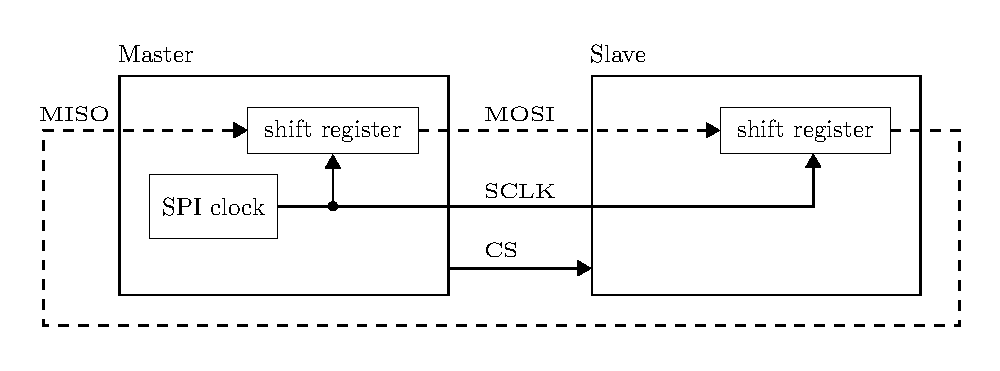
\includegraphics[width=0.8\textwidth]{spi_diagram}
        \caption{Diagrama conceptual del bus SPI.}
        \label{fig:spi_diagram}
    \end{figure}    

    Además de las líneas MOSI, MISO y SCLK, un dispositivo esclavo también puede tener una entrada de selección de chip activa en bajo, SS (para Slave Select). En otros casos también puede tener el nombre de  CS (para Chip-Select). Se puede utilizar para que el maestro seleccione el dispositivo esclavo deseado si hay varios dispositivos esclavos en el bus. Muchos dispositivos SPI también utilizan CS para ciertas funcionalidades de control y no se puede omitir, incluso en una configuración de un solo esclavo.

    \subsection{Configuración de múltiples dispositivos}

    El estándar SPI admite una configuración múltiple-esclavo, en la que un dispositivo maestro puede controlar más de un dispositivo esclavo. Existen dos esquemas básicos, que son la configuración en paralelo y la configuración en cadena.

    La configuración en paralelo utiliza una línea CS dedicada para cada dispositivo esclavo, como se muestra en la Figura \ref{fig:spi_parallel}. Una línea CS funciona como señal de selección de chip y el maestro puede seleccionar el dispositivo deseado activando la línea correspondiente. Esta configuración puede acomodar un maestro y dispositivos esclavos independientes. Dado que las líneas MISO de los esclavos están unidas, la línea MISO debe ser controlada por un buffer de tres estados y su salida debe estar en un estado de alta impedancia cuando el dispositivo esclavo no está seleccionado. 

    \begin{figure}[hbtp]
      \centering
      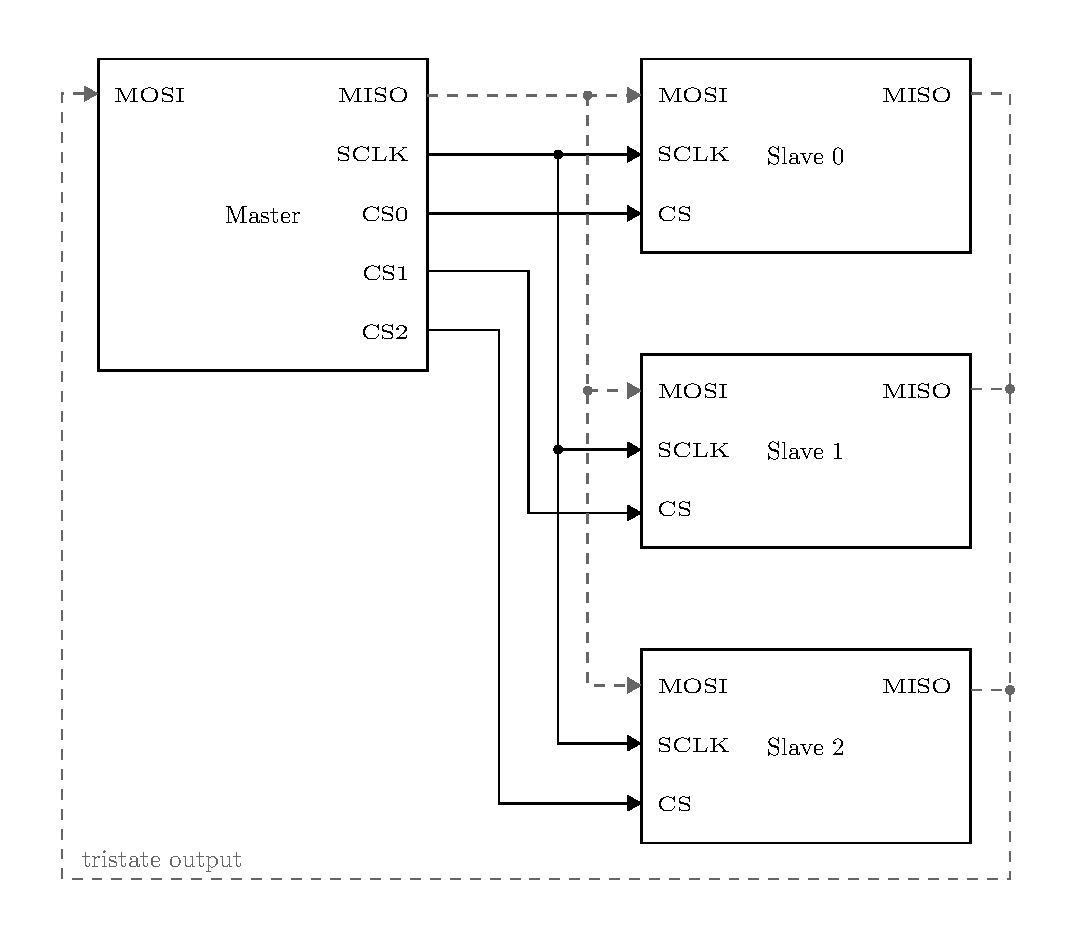
\includegraphics[width=0.8\textwidth]{spi_parallel}
      \caption{Configuración en paralelo de bus SPI.}
      \label{fig:spi_parallel}
    \end{figure}    

    La configuración en cadena conecta las líneas MOSI y MISO en una cadena en cascada, como se muestra en la Figura \ref{fig:spi_chain}. Se utiliza una única línea CS para controlar todos los dispositivos esclavos. Conceptualmente, la cadena forma un gran registro de desplazamiento y los datos se transfieren en serie de dispositivo a dispositivo. Los dispositivos de esta configuración deben ser cooperativos y seguir el mismo protocolo para transmitir, insertar y extraer bytes de datos.

    \begin{figure}[hbtp]
      \centering
      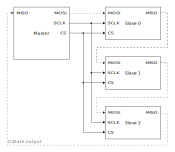
\includegraphics[width=0.8\textwidth]{spi_chain}
      \caption{Configuración en cadena de bus SPI.}
      \label{fig:spi_chain}
    \end{figure}    


    \subsection{Sincronización del controlador}

    El bus SPI utiliza los flancos del reloj SPI (SCLK) para controlar y sincronizar la transferencia de bits de los datos. Para aclarar la explicación, se definen dos actividades durante una transferencia de bits: enviar (es decir, desplazar) un nuevo bit a la línea de datos y muestrear (es decir, capturar) un bit de la línea de datos. El envío y el muestreo se completan en el mismo ciclo de reloj SPI, pero ocurren en flancos de reloj opuestos.
    En la Figura \ref{fig:spi_timing_diagram} se muestra un diagrama de tiempos representativo. Inicialmente, el bus está inactivo y la línea SCLK está en 0. En $t_{0}$, el maestro activa CS y el esclavo designado coloca el primer bit de datos (bit 7) en la línea MISO. En $t_{1}$, el maestro inicia el reloj SPI y envía el bit b7 en la línea MOSI.
Dado que la primera mitad del periodo del reloj SPI es 0, el valor en SCLK permanece sin cambios. El tiempo que transcurre entre $t_{0}$ y $t_{1}$ puede ser muy pequeño o incluso cero. En $t_{2}$, el maestro sube el reloj SPI y avanza a la segunda mitad del periodo del reloj. En el flanco de transición de 0 a 1, el maestro muestrea los datos en MISO y el esclavo los datos en MOSI. 
     En $t_{3}$, se completa el primer ciclo de reloj SPI. El maestro comienza el segundo periodo de reloj SPI y baja SCLK. Tanto el maestro como el esclavo envían nuevos bits a la línea de datos. En $t_{4}$, el maestro vuelve a subir SCLK y tanto el maestro como el esclavo muestrean los nuevos bits de datos. Las actividades de transmisión y muestreo se repiten hasta que se transfieren ocho bits de datos. Los últimos datos se muestrean en $t_{5}$ y SCLK vuelve a 0 en $t_{6}$. En $t_{7}$, el maestro desactiva CS. Cabe destacar que todos los muestreos se realizan en los flancos ascendentes de SCLK y todas las transmisiones (excepto la inicial) se realizan en los flancos descendentes de SCLK.

    \begin{figure}[hbtp]
      \centering
      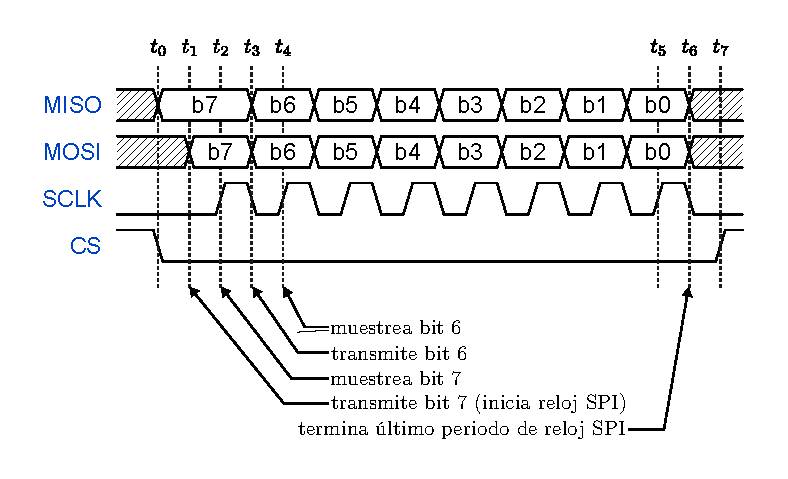
\includegraphics[width=0.8\textwidth]{spi_timing_diagram}
      \caption{Diagrama de tiempos representativo de una transferencia de datos SPI.}
      \label{fig:spi_timing_diagram}
    \end{figure}

    \subsection{Modos de operación}

    El modo de operación del SPI define las relaciones entre los flancos del reloj SPI y las actividades de envío y muestreo en las líneas de datos. Hay cuatro modos. Los modos dependen de dos parámetros, que son la polaridad del reloj (abreviado como CPOL, Clock Polarity) y la fase del reloj (abreviado como CPHA, Clock Phase). La polaridad del reloj se define como el valor de SCLK cuando está en reposo, que puede ser 0 o 1. La fase del reloj es más difícil de definir. Una interpretación es si un flanco del reloj se utiliza para enviar el primer bit de datos. Si CPHA es 1, el maestro conduce el bit en el primer flanco de transición. Si CPHA es 0, el maestro envía el bit en el flanco de transición cero, inmediatamente cuando CS se activa (lo que significa que no hay flanco o no en el primer flanco).

    Basándose en los dos parámetros, los modos de operación del SPI se definen como sigue:

    \begin{table}[h!]
      \caption{Modos de operación del SPI.}
      \begin{center}
      \resizebox{\textwidth}{!}{
        \begin{NiceTabular}{|c|c|c|c|c|}
          \hline
          \textbf{Modos SPI} & \textbf{Clock polarity} & \textbf{Clock phase } & \textbf{Los datos de desplazan en } & \textbf{Los datos se muestrean en }\\
                             & \textbf{(CPOL)}         & \textbf{(CPHA)}       &                                     & \\
          \hline
          0 & 0 & 0 & bajada SCLK, y cuando CS se activa & subida SCLK \\
          1 & 0 & 1 & subida SCLK & bajada SCLK \\
          2 & 1 & 0 & subida SCLK, y cuando CS se activa & bajada SCLK \\
          3 & 1 & 1 & bajada SCLK & subida SCLK \\
          \hline
        \end{NiceTabular}
      }
      \label{tab:spi_modes}
      \end{center}
    \end{table}

    Observe que el diagrama de tiempos de la Figura \ref{fig:spi_timing_diagram} corresponde al modo 0, ya que SCLK es 0 cuando está inactivo y el primer bit no es transmitido por el primer flanco de transición.

    El diagrama de tiempo de los cuatro modos se muestra en la Figura \ref{fig:spi_timing_diagram_modes}. El modo 0 es el modo más comúnmente utilizado. En este modo, el valor en reposo es 0 y el ciclo del reloj comienza con 0. Dado que el valor en reposo y el valor inicial del reloj son los mismos, el primer bit de datos se transmite antes del primer flanco de transición. En el modo 1, el valor en reposo también es 0, pero el ciclo del reloj comienza con 1. El valor inicial de 1 lleva a una transición de 0 a 1, por lo tanto, el primer bit se transmite en el primer flanco. Es importante notar que en estos dos modos, el período del reloj y el tiempo de inicio son los mismos, pero sus valores están fuera de fase.

    \begin{figure}[!h]
      \centering
      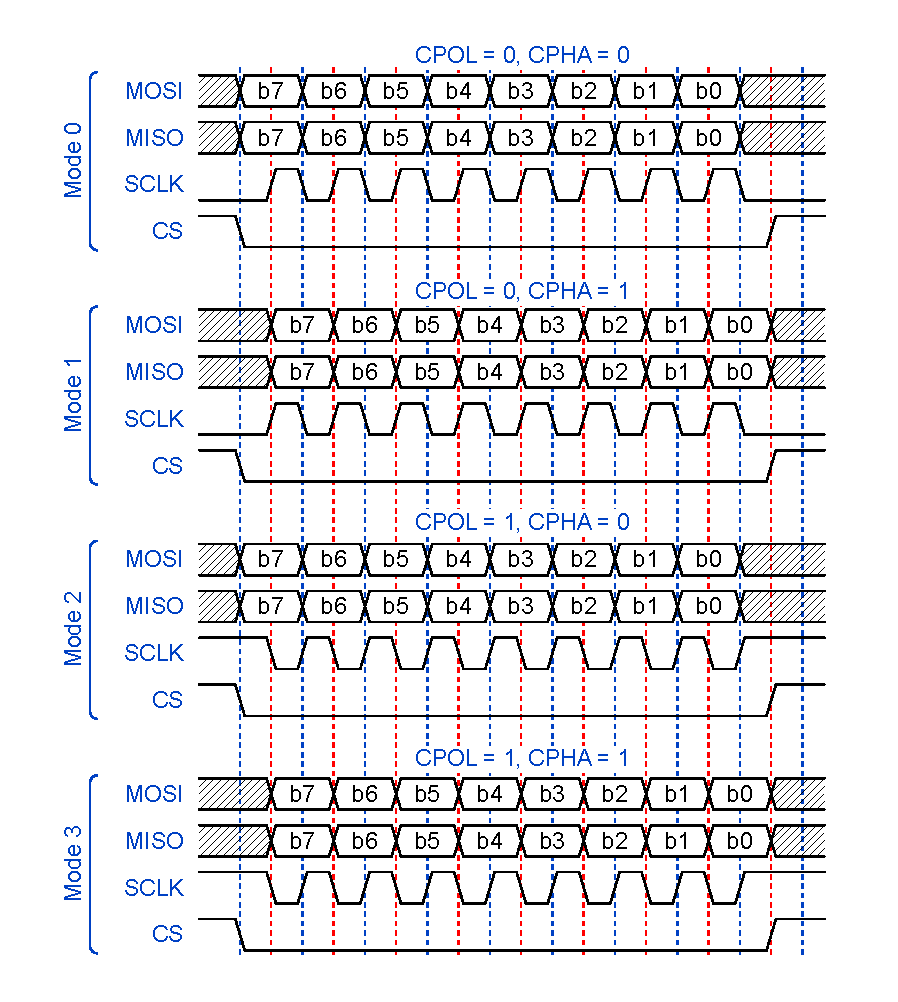
\includegraphics[width=0.85\textwidth]{spi_timing_diagram_modes}
      \caption{Diagrama de tiempos de los diferentes modos SPI.}
      \label{fig:spi_timing_diagram_modes}
    \end{figure}

    El valor en reposo de SCLK en los modos 2 y 3 es 1. La forma de onda de SCLK en el modo 2 es exactamente opuesta a la del modo 0, y la forma de onda en el modo 3 es exactamente opuesta a la del modo 1. Nuevamente, es importante destacar que el período del reloj y el tiempo de inicio son los mismos para todos los modos.

    \subsection{Aspectos indefinidos}

    La interfaz SPI fue desarrollada por Motorola y se ha convertido en un estándar de facto. No existe un organismo rector u organización que supervise este estándar. Varios aspectos importantes no están definidos en el estándar.

    El primer aspecto es el uso de la señal CS. La señal CS actúa principalmente como una señal de habilitación o selección de chip. Un dispositivo esclavo se desactiva si su señal CS no está activa. En muchos dispositivos, la señal CS también funciona como una señal de control. El intercambio de datos se realiza transacción por transacción:

    \begin{itemize}
      \item El maestro activa CS.
      \item El maestro y el esclavo seleccionado transfieren bits de datos.
      \item El maestro desactiva CS.
    \end{itemize}

    Una transacción se muestra en la Figura \ref{fig:spi_timing_diagram_aspects}. Las transiciones causadas por la activación y desactivación de CS se utilizan para activar ciertas acciones, como enviar un bit o capturar datos en paralelo, en el dispositivo esclavo. Esto implica que CS debe estar conectado al maestro, incluso si solo hay un dispositivo esclavo; es decir, simplemente conectarlo a 0 no funcionará. El estándar SPI no define explícitamente el papel de la señal CS ni el protocolo en la transacción. Además, los requisitos de temporización como el tiempo de preparación de CS ($\text{t}_{\text{SS\_SETUP}}$), que es el intervalo entre la activación de CS y el inicio del reloj, el tiempo de retención de CS ($\text{t}_{\text{SS\_HOLD}}$), que es el intervalo entre la desactivación de CS y la terminación del reloj, y el tiempo de cambio entre dos transacciones ($\text{t}_{\text{SS\_TURN}}$) no esta especificado.

    \begin{figure}[!h]
      \centering
      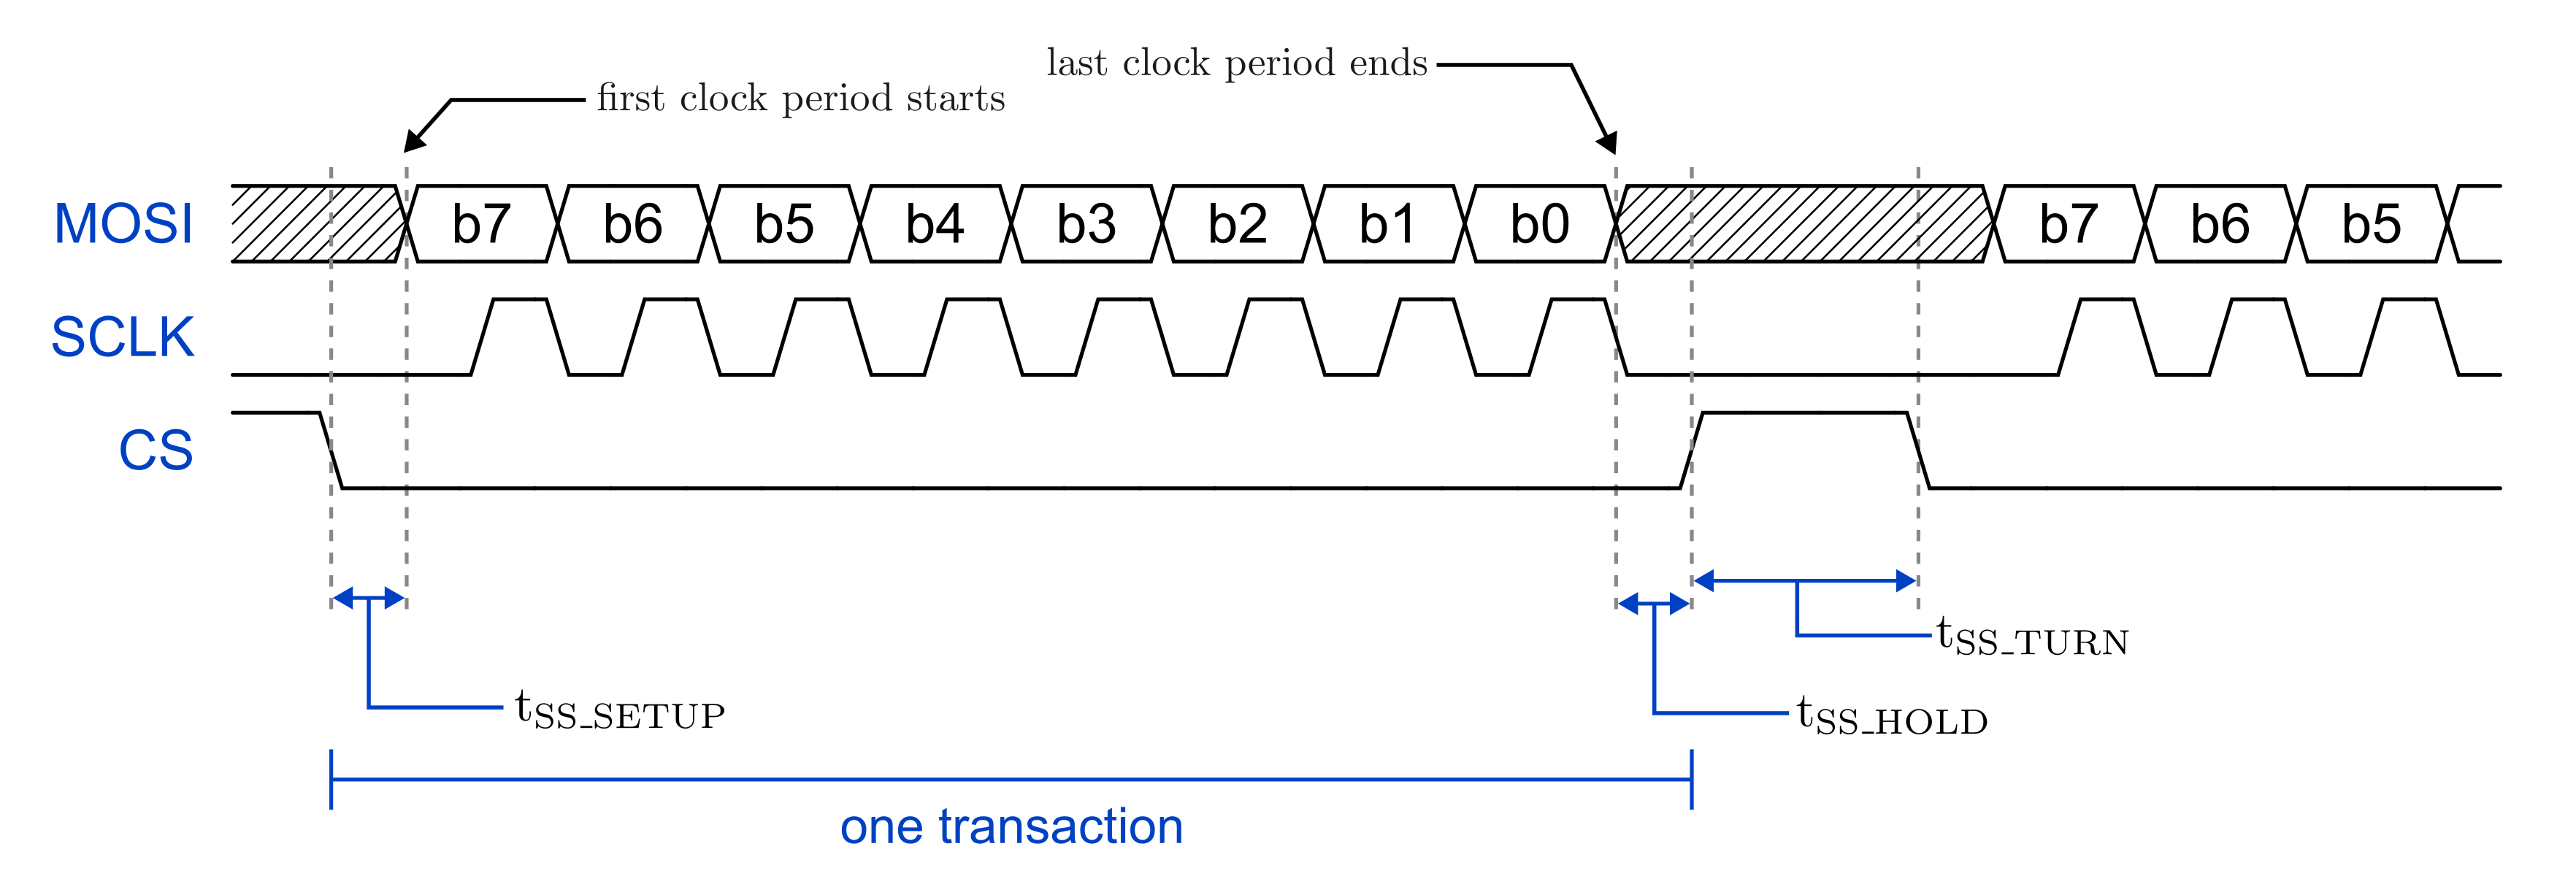
\includegraphics[width=0.95\textwidth]{spi_timing_diagram_aspects}
      \caption{Diagrama de tiempos con aspectos indefinidos, SPI modo 0.}
      \label{fig:spi_timing_diagram_aspects}
    \end{figure}

    El segundo aspecto indefinido es el número de bits en un intercambio de datos. En la Figura \ref{fig:spi_timing_diagram} se transfieren ocho bits. Sin embargo, el estándar SPI no especifica el número de bits transferidos en una transacción.

    Finalmente, el estándar SPI no especifica el orden de bits de la transmisión, es decir, si se transfiere primero el bit mas significactivo (MSB) o el bit menos significativo (LSB) de un byte de datos o de una palabra de datos. El MSB se utiliza comúnmente, pero no está garantizado.

    Debido a estos aspectos indefinidos, debemos consultar la hoja de datos del dispositivo y adaptar el acceso para cada dispositivo. Esto suele hacerlo el controlador de software y el programa de aplicación.

	\section{Digital-To-Analog Converters}

	\section{Analog-To-Digital Converters}

  Los convertidores analógico-digitales (ADC) traducen las magnitudes analógicas, características de la mayoría de los fenómenos del «mundo real», a lenguaje digital, utilizado en el tratamiento de la información, la informática, la transmisión de datos y los sistemas de control. Los convertidores de digital a analógico (DAC) se utilizan para transformar los datos transmitidos o almacenados, o los resultados del procesamiento digital, de nuevo en variables del «mundo real» para su control, visualización de información o procesamiento analógico posterior.
	
